%!TEX program = xelatex
\documentclass[hyperref,UTF8,12pt]{sdnubachelor}

\begin{document}
	
%---信息部分-------------------------------------------------------------------------------
	\sdnutitle{人机博弈机制分析与算法研究}{English Title}
	\sdnuauthor{光头强}{201411010300}
	\sdnumentor{熊大}
	\sdnuinfo{信息科学与工程学院}{计算机科学与技术}{计信本1401}
	\sdnudate{2018}{2}{15}
	\sdnukeyw{关键字1\quad 关键字2\quad 关键字3\quad 关键字4}{key1,key2,key3,key4}
	\sdnuwdnum{66666} %论文字数
	
%---封面部分,注释\begin{titlepage}
	\vspace*{3mm}
	\begin{center}
		
\includegraphics[width=0.77\textwidth,trim=8 0 0 0,clip]{data/resource/logo.jpg}
	\end{center}
	\vspace*{1cm}
	\fontsize{50pt}{24pt}
	\centering
	\textbf{本}\hfill\textbf{科}\hfill\textbf{毕}\hfill\textbf{业}\hfill\textbf{论}\hfill\textbf{文}
	\\
	\vspace*{7.7cm}
	\zihao{3}
	论文题目:\underline{\makebox[\nlength]{\sdnutitlechs}}\\\vspace*{1mm}
	学生姓名:\underline{\makebox[\nlength]{\sdnuauthorchs}}\\\vspace*{1mm}
	学~ \quad ~号:\underline{\makebox[\nlength]{\sdnuauthorid}}\\\vspace*{1mm}
	专~ \quad ~业:\underline{\makebox[\nlength]{\sdnumajorchs}}\\\vspace*{1mm}
	指导教师:\underline{\makebox[\nlength]{\sdnumentorchs}}\\\vspace*{1mm}
	学~ \quad ~院:\underline{\makebox[\nlength]{\sdnucollegechs}}\\\vspace*{2.2cm}
	\sdnuyear 年\sdnumon 月\sdnuday 日
\end{titlepage}一行可以不编译封面---------------------------
	{
		\newlength{\nlength}
		\setlength{\nlength}{7.8cm}	%封面题目线长度,根据题目长短自行调整,默认7.8cm
		\begin{titlepage}
	\vspace*{3mm}
	\begin{center}
		
\includegraphics[width=0.77\textwidth,trim=8 0 0 0,clip]{data/resource/logo.jpg}
	\end{center}
	\vspace*{1cm}
	\fontsize{50pt}{24pt}
	\centering
	\textbf{本}\hfill\textbf{科}\hfill\textbf{毕}\hfill\textbf{业}\hfill\textbf{论}\hfill\textbf{文}
	\\
	\vspace*{7.7cm}
	\zihao{3}
	论文题目:\underline{\makebox[\nlength]{\sdnutitlechs}}\\\vspace*{1mm}
	学生姓名:\underline{\makebox[\nlength]{\sdnuauthorchs}}\\\vspace*{1mm}
	学~ \quad ~号:\underline{\makebox[\nlength]{\sdnuauthorid}}\\\vspace*{1mm}
	专~ \quad ~业:\underline{\makebox[\nlength]{\sdnumajorchs}}\\\vspace*{1mm}
	指导教师:\underline{\makebox[\nlength]{\sdnumentorchs}}\\\vspace*{1mm}
	学~ \quad ~院:\underline{\makebox[\nlength]{\sdnucollegechs}}\\\vspace*{2.2cm}
	\sdnuyear 年\sdnumon 月\sdnuday 日
\end{titlepage}
	}

%---论文内容摘要信息页,注释\newpage
\pagestyle{empty}
\vspace*{-5mm}
{
	\centering
	\noindent\zihao{2}\textbf{山东师范大学本科毕业论文摘要}\\
	\vspace*{2mm}
	\zihao{-4}\textbf{学院:\resdnucollegechs \hfill 专业:\resdnumajorchs \hfill 班级:\resdnuclasschs}\\
	\vspace*{3mm}
	\centerline{
		\extrarowsep = 3mm
		\begin{tabu} to 1.02\textwidth {|X[c]|X[c]|X[c]|X[c]|X[c]|X[c]|X[c]|}
			\tabucline-
			\rowfont{\zihao{-4}}姓名&\sdnuauthorchs&学号&\multicolumn{2}{c|}{\sdnuauthorid}&指导教师&\sdnumentorchs\\
			\tabucline-
			\rowfont{\zihao{-4}}论文题目&\multicolumn{6}{l|}{\sdnutitlechs}\\
			\tabucline-
			\rowfont{\zihao{-4}}关键词&\multicolumn{4}{l|}{{\etkwzihao\sdnukeywchs}}&论文字数&\wordcount\\
			\tabucline-
			\rowfont{\zihao{-4}}\multicolumn{7}{|c|}{\makecell*[{}{p{1.02\textwidth}}]{\vspace*{-2mm} 内容摘要:\\ \vspace*{-1mm} \setlength{\baselineskip}{20pt} \cabstchs}}\\
			\tabucline-
			\rowfont{\zihao{-4}}成绩&\cabstgrade&\multicolumn{2}{c|}{学院负责人(签名)}&&\multicolumn{2}{c|}{\cabsty 年\cabstm 月\cabstd 日}\\
			\tabucline-
			\tabuphantomline
		\end{tabu}
	}
}
\vspace*{3mm}
\noindent\zihao{5}\textbf{注:文科论文摘要不少于500字,理科不少于300字。}\\
本页一式两份,一份装入学生档案,一份由学院保存
可不编译此页--------------------
{
	\resdnuinfo{\sdnucollegechs}{\sdnumajorchs}{\sdnuclasschs} %学院、专业、班级信息重述,如不符合排版要求,可在此进行简称替换
	\newcommand{\etkwzihao}{\zihao{-4}}	%表格中关键词字号自定义,防止关键词过多造成的排版混乱
	\cabst{这里是摘要内容,由于tabu环境请使用双反斜换行,使用qquad进行段首缩进,qquad后不要忘记空格与中文字符间开,请适当调整内容量保证表格排版美观。 \\ \\ \\ \\ \\ \\ \\ \\ \\ \\ \\ \\ \\ \\ \\ \\ \\ \\ \\ \\ \\}{\qquad}{\qquad}{\qquad}{\qquad} %依次填入:内容摘要、成绩、年、月、日,不填写请用\qquad代替
	\newpage
\pagestyle{empty}
\vspace*{-5mm}
{
	\centering
	\noindent\zihao{2}\textbf{山东师范大学本科毕业论文摘要}\\
	\vspace*{2mm}
	\zihao{-4}\textbf{学院:\resdnucollegechs \hfill 专业:\resdnumajorchs \hfill 班级:\resdnuclasschs}\\
	\vspace*{3mm}
	\centerline{
		\extrarowsep = 3mm
		\begin{tabu} to 1.02\textwidth {|X[c]|X[c]|X[c]|X[c]|X[c]|X[c]|X[c]|}
			\tabucline-
			\rowfont{\zihao{-4}}姓名&\sdnuauthorchs&学号&\multicolumn{2}{c|}{\sdnuauthorid}&指导教师&\sdnumentorchs\\
			\tabucline-
			\rowfont{\zihao{-4}}论文题目&\multicolumn{6}{l|}{\sdnutitlechs}\\
			\tabucline-
			\rowfont{\zihao{-4}}关键词&\multicolumn{4}{l|}{{\etkwzihao\sdnukeywchs}}&论文字数&\wordcount\\
			\tabucline-
			\rowfont{\zihao{-4}}\multicolumn{7}{|c|}{\makecell*[{}{p{1.02\textwidth}}]{\vspace*{-2mm} 内容摘要:\\ \vspace*{-1mm} \setlength{\baselineskip}{20pt} \cabstchs}}\\
			\tabucline-
			\rowfont{\zihao{-4}}成绩&\cabstgrade&\multicolumn{2}{c|}{学院负责人(签名)}&&\multicolumn{2}{c|}{\cabsty 年\cabstm 月\cabstd 日}\\
			\tabucline-
			\tabuphantomline
		\end{tabu}
	}
}
\vspace*{3mm}
\noindent\zihao{5}\textbf{注:文科论文摘要不少于500字,理科不少于300字。}\\
本页一式两份,一份装入学生档案,一份由学院保存

}

%---目录生成部分,此部分无需在意------------------------------------------------------------
	{
		\begin{titlepage}
			\pagestyle{empty}
			\tableofcontents
		\end{titlepage}
	}
	
%---中英文摘要部分-------------------------------------------------------------------------
	{
		\abstract{在此键入你的中文摘要,可以使用par换段或双反斜强制换行。}{Please input your english abstract here.}
		{
	\phantomsection
	\addcontentsline{toc}{section}{中文摘要}
	\centering
	\noindent\textbf{\zihao{3}\sdnutitlechs}\\
	\vspace*{5mm}
	\textbf{\zihao{4}摘~要}\\
	\vspace*{5mm}
}
\abstractchs
\par
\vspace*{5mm}
\noindent\textbf{关键词:}\sdnukeywchs
\newpage
{
	\phantomsection
	\addcontentsline{toc}{section}{英文摘要}
	\centering
	\noindent\textbf{\zihao{3}\sdnutitleen}\\
	\vspace*{5mm}
	\textbf{\zihao{4}ABSTRACT}\\
	\vspace*{5mm}
}
\abstracten
\par
\vspace*{5mm}
\noindent\textbf{KEY WORDS: }\sdnukeywen
\newpage
	}

%---正文部分,编辑正文请前往./data/resource/article.tex-------------------------------------
	{
		\setlength{\abovedisplayskip}{1pt}
		\setlength{\belowdisplayskip}{1pt}
		\setlength{\belowcaptionskip}{-10pt}
		\section{引言}
	秩序是社会生活的根本问题,它是社会生活得以可能的深刻根据,与一般社会理论有着深刻的关联,构成一般社会理论或社会哲学的核心主题。\par
	参考文献引用示例\upcite{1,3}。
\section{关于创新的思考}
	\subsection{秩序问题的创新}
	\subsubsection{……}
\section{社会哲学的主题}
	\subsection{示例}
	插图示例:测试图例如图\ref{test-pic}所示,建议使用以htbp为顺序的浮动格式,减少文中“上图”、“下图”之类的描述,转而使用“图X”的描述方式,如必须如前者描述,请仅使用h控制图片浮动。请将文件放置在data/img/文件夹中,图片目录已自动索引,此处不建议也请勿省略后缀名。
	\begin{figure}[htbp]
		\centering
		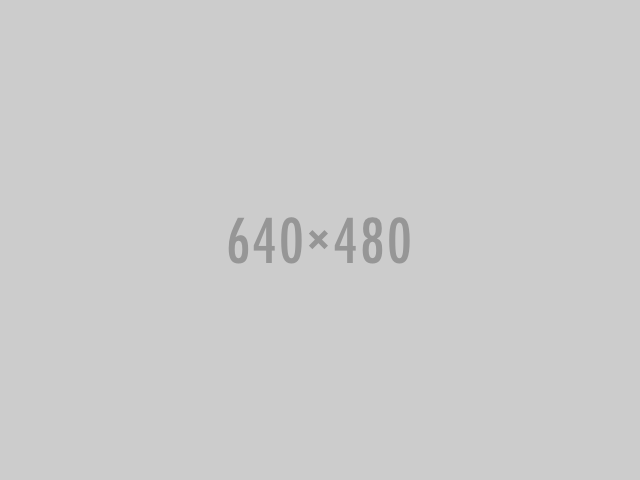
\includegraphics[width=0.5\textwidth]{test.png}
		\caption{示例图片\label{test-pic}}
	\end{figure}
	\par
	表格插入示例:测试表格如表\ref{test-table}所示,此处建议使用三线表格,更加复杂的表格(如自动伸缩表格)请使用tabularx或tabu环境,相关宏包已引入。
	\begin{table}[htbp]
		\centering
		\begin{tabular}{ccccc}
			\toprule
			\multirow{2}*{姓名}&\multicolumn{2}{c}{森林}&\multicolumn{2}{c}{房屋}\\
			\cmidrule{2-5}
			&熊大&熊二&光头强&肥波\\
			\midrule
			成绩&97&98&99&70\\
			\bottomrule
		\end{tabular}
		\caption{测试表格\label{test-table}}
	\end{table}
	\par
	定理环境示例:定理\ref{bear-thm}是熊出没定理。
	\begin{theorem}[熊出没定理]\label{bear-thm}
		熊大和熊二以及光头强是好朋友。
	\end{theorem}
	定义环境示例:定义\ref{bear-def}是Bear定义。
	\begin{definition}[Bear定义]\label{bear-def}
		将熊二的弟弟定义为熊三。
	\end{definition}
	证明环境示例:
	\begin{proof}[定理\ref{bear-thm}的证明]
		这里是证明环境。
	\end{proof}
	公式环境示例:公式\ref{mass-energy equation}为爱因斯坦质能方程。
	\begin{equation}\label{mass-energy equation}
		E=mc^{2}
	\end{equation}
	质能方程$E=mc^{2}$,$E$表示能量,$m$代表质量,而$c$则表示光速(常量,$c=299792.458km/s$)。由阿尔伯特·爱因斯坦提出。$$E=mc^{2}$$该方程主要用来解释核变反应中的质量亏损和计算高能物理中粒子的能量。这也导致了德布罗意波和波动力学的诞生。
	
	}
	
%---参考文献引入部分,修改参考文献请修改./data/resource/bibliography.tex--------------------
	{
		\newpage
\phantomsection
\addcontentsline{toc}{section}{参考文献}
\begin{thebibliography}{99}
	\zihao{5}
	\bibitem{1}
		马尔科姆•沃斯特.现代社会学理论[M].杨善华译.北京:华夏出版社,2000.
	\bibitem{2}
		杰弗里•亚历山大.社会学二十讲:二战以来的理论发展[M].贾春增,董天民,等译.北京:华夏出版社,2000.
	\bibitem{3}
		万俊人.信用伦理及其现代解释[J].孔子研究,2002,(5).
\end{thebibliography}
	}

%---附录引入部分,修改附录内容请修改./data/resource/appendix.tex,无需附录请注释\include部分--
	{
		\newpage
\phantomsection
\addcontentsline{toc}{section}{附录}
\section*{[附录]}
\vspace*{-2mm}
\zihao{5}
\setlength{\baselineskip}{25pt}

这里是附录内容,附录等级为section,若使用下级内容,请在附录内使用subsection*开始下级。

代码环境lstlisting,代码\ref{testcode1}为示例代码1,代码\ref{testcode2}为示例代码2:
\begin{lstlisting}[caption={代码示例1\label{testcode1}}]
int main(int argc,char **argv){
	printf("Hello World!\n");
	return 0;
}
\end{lstlisting}
\begin{lstlisting}[caption={代码示例2\label{testcode2}}]
int main(int argc,char **argv){
	printf("Hello World!\n");
	return 0;
}
\end{lstlisting}
	}

%---指导教师意见部分,注释\newpage
\pagestyle{empty}
\vspace*{-5mm}
{
	\centering
	\noindent\zihao{3}\textbf{指导教师意见}\\
	\vspace*{2mm}
	\centerline{
		\begin{tabu} to 1.02\textwidth {|X[c]|}
			\tabucline-
			\rowfont{\zihao{-4}}\multicolumn{1}{|c|}{\makecell*[{}{p{1.02\textwidth}}]{\guidancechs\\ \\ \qquad 成绩:\guidancegrade \\ \\ \qquad \hfill 指导教师(签名):\quad\qquad\qquad\qquad\qquad\qquad\qquad\qquad \\ \qquad \hfill \guidancey 年\guidancem 月\guidanced 日\qquad\qquad\qquad\qquad\qquad\qquad\qquad\qquad}}\\
			\tabucline-
		\end{tabu}
	}
}
\vspace*{2mm}
\noindent\zihao{-4}注:成绩按优、良、中、合格、不合格五级分制计。可不编译此页---------------------
	{
		\guidance{(包括选题的意义,资料收集或实验方法、数据处理等方面的能力,论证或实验是否合理,主要观点或结果是否正确,有何独到的见解或新的方法,基础理论、专业知识的掌握程度及写作水平等,并就该论文是否达到本科毕业论文水平做出评价) \\ \\ \\ \\ \\ \\ \\ \\ \\ \\ \\ \\ \\ \\ \\ \\ \\ \\ \\ \\ \\ \\ \\ \\ \\ \\}{\qquad}{\qquad}{\qquad}{\qquad}	%依次填入:指导意见、成绩、年、月、日,不填写请用\qquad代替
		\newpage
\pagestyle{empty}
\vspace*{-5mm}
{
	\centering
	\noindent\zihao{3}\textbf{指导教师意见}\\
	\vspace*{2mm}
	\centerline{
		\begin{tabu} to 1.02\textwidth {|X[c]|}
			\tabucline-
			\rowfont{\zihao{-4}}\multicolumn{1}{|c|}{\makecell*[{}{p{1.02\textwidth}}]{\guidancechs\\ \\ \qquad 成绩:\guidancegrade \\ \\ \qquad \hfill 指导教师(签名):\quad\qquad\qquad\qquad\qquad\qquad\qquad\qquad \\ \qquad \hfill \guidancey 年\guidancem 月\guidanced 日\qquad\qquad\qquad\qquad\qquad\qquad\qquad\qquad}}\\
			\tabucline-
		\end{tabu}
	}
}
\vspace*{2mm}
\noindent\zihao{-4}注:成绩按优、良、中、合格、不合格五级分制计。
	}

%---评阅人意见部分,注释\newpage
\pagestyle{empty}
\vspace*{-5mm}
{
	\centering
	\noindent\zihao{3}\textbf{评阅人意见}\\
	\vspace*{2mm}
	\centerline{
		\begin{tabu} to 1.02\textwidth {|X[c]|}
			\tabucline-
			\rowfont{\zihao{-4}}\multicolumn{1}{|c|}{\makecell*[{}{p{1.02\textwidth}}]{\reviewerpchs\\ \\ \qquad 成绩:\reviewerpgrade \\ \\ \qquad \hfill 评阅人(签名):\quad\qquad\qquad\qquad\qquad\qquad\qquad\qquad \\ \qquad \hfill \reviewerpy 年\reviewerpm 月\reviewerpd 日\qquad\qquad\qquad\qquad\qquad\qquad\qquad\qquad}}\\
			\tabucline-
		\end{tabu}
	}
}
\vspace*{2mm}
\noindent\zihao{-4}注:成绩按优、良、中、合格、不合格五级分制计。可不编译此页-----------------------
	{
		\reviewerp{(包括选题的意义,资料收集或实验方法、数据处理等方面的能力,论证或实验是否合理,主要观点或结果是否正确,有何独到的见解或新的方法,基础理论、专业知识的掌握程度及写作水平等,并就该论文是否达到本科毕业论文水平做出评价) \\ \\ \\ \\ \\ \\ \\ \\ \\ \\ \\ \\ \\ \\ \\ \\ \\ \\ \\ \\ \\ \\ \\ \\ \\ \\}{\qquad}{\qquad}{\qquad}{\qquad}	%依次填入:评阅意见、成绩、年、月、日,不填写请用\qquad代替
		\newpage
\pagestyle{empty}
\vspace*{-5mm}
{
	\centering
	\noindent\zihao{3}\textbf{评阅人意见}\\
	\vspace*{2mm}
	\centerline{
		\begin{tabu} to 1.02\textwidth {|X[c]|}
			\tabucline-
			\rowfont{\zihao{-4}}\multicolumn{1}{|c|}{\makecell*[{}{p{1.02\textwidth}}]{\reviewerpchs\\ \\ \qquad 成绩:\reviewerpgrade \\ \\ \qquad \hfill 评阅人(签名):\quad\qquad\qquad\qquad\qquad\qquad\qquad\qquad \\ \qquad \hfill \reviewerpy 年\reviewerpm 月\reviewerpd 日\qquad\qquad\qquad\qquad\qquad\qquad\qquad\qquad}}\\
			\tabucline-
		\end{tabu}
	}
}
\vspace*{2mm}
\noindent\zihao{-4}注:成绩按优、良、中、合格、不合格五级分制计。
	}

%---答辩意见以及学院委员会意见,注释\newpage
\pagestyle{empty}
\vspace*{-5mm}
{
	\centering
	\noindent\zihao{3}\textbf{答辩委员会意见}\\
	\vspace*{2mm}
	\centerline{
		\begin{tabu} to 1.02\textwidth {|X[c]|}
			\tabucline-
			\rowfont{\zihao{-4}}\multicolumn{1}{|c|}{\makecell*[{}{p{1.02\textwidth}}]{\replychs\\ \\ \qquad 成绩:\replygrade \\ \\ \qquad \hfill 答辩委员会主任(签名):\qquad\qquad\qquad\qquad\qquad\qquad\qquad \\ \qquad \hfill \replyy 年\replym 月\replyd 日\qquad\qquad\qquad\qquad\qquad\qquad\qquad\qquad}}\\
			\tabucline-
		\end{tabu}
	}
	\vspace*{5mm}
	\noindent\zihao{-4}\textbf{学院学位分委员会意见}\\
	\vspace*{2mm}
	\centerline{
		\begin{tabu} to 1.02\textwidth {|X[c]|}
			\tabucline-
			\rowfont{\zihao{-4}}\multicolumn{1}{|c|}{\makecell*[{}{p{1.02\textwidth}}]{\\ \\ \\ \\ \qquad 成绩:\xuefengrade \\ \\ \qquad \hfill 学位分委员会主任(签名):\qquad\qquad\qquad(公章) \\ \qquad \hfill \replyy 年\replym 月\replyd 日\qquad\qquad\qquad\qquad\qquad\qquad\qquad\qquad}}\\
			\tabucline-
		\end{tabu}
	}
}
\vspace*{2mm}
\noindent\zihao{-4}注:成绩按优、良、中、合格、不合格五级分制计。可不编译此页------------
	{
		\reply{(应根据论文内容和答辩情况,并参考指导教师意见、评阅人意见对论文的综合水平做出具体评价) \\ \\ \\ \\ \\ \\ \\ \\ \\ \\ \\ \\ \\ \\ \\ \\ \\}{\qquad}{\qquad}{\qquad}{\qquad}	%依次填入:答辩意见、成绩、年、月、日,不填写请用\qquad代替
		\xuefen{\qquad}{\qquad}{\qquad}{\qquad}	%依次填入:学院学位分委员会成绩、年、月、日,不填写请用\qquad代替
		\newpage
\pagestyle{empty}
\vspace*{-5mm}
{
	\centering
	\noindent\zihao{3}\textbf{答辩委员会意见}\\
	\vspace*{2mm}
	\centerline{
		\begin{tabu} to 1.02\textwidth {|X[c]|}
			\tabucline-
			\rowfont{\zihao{-4}}\multicolumn{1}{|c|}{\makecell*[{}{p{1.02\textwidth}}]{\replychs\\ \\ \qquad 成绩:\replygrade \\ \\ \qquad \hfill 答辩委员会主任(签名):\qquad\qquad\qquad\qquad\qquad\qquad\qquad \\ \qquad \hfill \replyy 年\replym 月\replyd 日\qquad\qquad\qquad\qquad\qquad\qquad\qquad\qquad}}\\
			\tabucline-
		\end{tabu}
	}
	\vspace*{5mm}
	\noindent\zihao{-4}\textbf{学院学位分委员会意见}\\
	\vspace*{2mm}
	\centerline{
		\begin{tabu} to 1.02\textwidth {|X[c]|}
			\tabucline-
			\rowfont{\zihao{-4}}\multicolumn{1}{|c|}{\makecell*[{}{p{1.02\textwidth}}]{\\ \\ \\ \\ \qquad 成绩:\xuefengrade \\ \\ \qquad \hfill 学位分委员会主任(签名):\qquad\qquad\qquad(公章) \\ \qquad \hfill \replyy 年\replym 月\replyd 日\qquad\qquad\qquad\qquad\qquad\qquad\qquad\qquad}}\\
			\tabucline-
		\end{tabu}
	}
}
\vspace*{2mm}
\noindent\zihao{-4}注:成绩按优、良、中、合格、不合格五级分制计。
	}

%---原封面表格部分,注释\begin{titlepage}
	\pagestyle{empty}
	\vspace*{-5mm}
	\zihao{4}\noindent\textbf{毕业论文内容介绍}\\
	\vspace*{-5mm}\\
	\centerline{
		\extrarowsep = 3mm
		\begin{tabu} to 1.02\textwidth {|X[c]|X[c]|X[c]|X[c]|X[c]|X[c]|}
			\tabucline-
			\rowfont{\zihao{5}}论文题目&\multicolumn{5}{l|}{\textbf{\sdnutitlechs}}\\
			\tabucline-
			\rowfont{\zihao{5}}选题时间&\selectdate&完成时间&\finishdate&论文字数&\wordcount\\
			\tabucline-
			\rowfont{\zihao{5}}关键词&\multicolumn{5}{l|}{\sdnukeywchs}\\
			\tabucline-
			\rowfont{\zihao{5}}\multicolumn{6}{|c|}{\makecell*[{}{p{1.02\textwidth}}]{\vspace*{-2mm} 论文题目的来源、理论和实践意义:\\ \vspace*{-1.5mm} \means}}\\
			\tabucline-
			\rowfont{\zihao{5}}\multicolumn{6}{|c|}{\makecell*[{}{p{1.02\textwidth}}]{\vspace*{-2mm} 论文的主要内容及创新点:\\ \vspace*{-1.5mm} \inovations}}\\
			\tabucline-
			\rowfont{\zihao{5}}附:论文&\multicolumn{5}{l|}{本人签名:\hfill \tableyear 年\tablemon 月\tableday 日}\\
			\tabucline-
			\tabuphantomline
		\end{tabu}
	}
\end{titlepage}一行可以不编译封面表格---------------
{
	\sdnupaperinfo{2017.10.25}{2018.02.25} %表头时间
	\sdnutabledate{\qquad}{\qquad}{\qquad} %表尾时间,不填写请用\qquad填充
	\sdnupaperov{
		\qquad 在此键入论文题目的来源、理论和实践意义,由于tabu环境请使用双反斜换行,使用qquad进行段首缩进,qquad后不要忘记空格与中文字符间开,请适当调整内容量保证表格排版美观。\\ \\ \\ \\ \\ \\ \\ \\ \\ \\ \\ \\ \\
	}{
		\qquad 在此键入论文的主要内容及创新点,由于tabu环境请使用双反斜换行,使用qquad进行段首缩进,qquad后不要忘记空格与中文字符间开,请适当调整内容量保证表格排版美观。\\ \\ \\ \\ \\ \\ \\ \\ \\ \\ \\ \\
	}
	\begin{titlepage}
	\pagestyle{empty}
	\vspace*{-5mm}
	\zihao{4}\noindent\textbf{毕业论文内容介绍}\\
	\vspace*{-5mm}\\
	\centerline{
		\extrarowsep = 3mm
		\begin{tabu} to 1.02\textwidth {|X[c]|X[c]|X[c]|X[c]|X[c]|X[c]|}
			\tabucline-
			\rowfont{\zihao{5}}论文题目&\multicolumn{5}{l|}{\textbf{\sdnutitlechs}}\\
			\tabucline-
			\rowfont{\zihao{5}}选题时间&\selectdate&完成时间&\finishdate&论文字数&\wordcount\\
			\tabucline-
			\rowfont{\zihao{5}}关键词&\multicolumn{5}{l|}{\sdnukeywchs}\\
			\tabucline-
			\rowfont{\zihao{5}}\multicolumn{6}{|c|}{\makecell*[{}{p{1.02\textwidth}}]{\vspace*{-2mm} 论文题目的来源、理论和实践意义:\\ \vspace*{-1.5mm} \means}}\\
			\tabucline-
			\rowfont{\zihao{5}}\multicolumn{6}{|c|}{\makecell*[{}{p{1.02\textwidth}}]{\vspace*{-2mm} 论文的主要内容及创新点:\\ \vspace*{-1.5mm} \inovations}}\\
			\tabucline-
			\rowfont{\zihao{5}}附:论文&\multicolumn{5}{l|}{本人签名:\hfill \tableyear 年\tablemon 月\tableday 日}\\
			\tabucline-
			\tabuphantomline
		\end{tabu}
	}
\end{titlepage}
}

\end{document}